\documentclass[t,aspectratio=169]{beamer}

\usepackage{soul}
\usepackage[utf8]{inputenc}

% ----------------------------------------------------------------------------------------------------------------------------------------

\title{
\includegraphics[width=45pt]{oepecsetlogo.png}\\(KTXFI2EBNF) Physics II. Lecture}

% \subtitle{1-4. lecture}

\author{Dr.~Gábor FACSKÓ, PhD\\\tiny Assistant Professor / Senior Research Fellow\\\textit{facsko.gabor@uni-obuda.hu}}

\institute{\Tiny Óbuda University, Faculty of Electrical Engineering, 1084 Budapest, Tavaszmező u. 17.\\Wigner Research Centre for Physics, Department of Space Physics and Space Technology, 1121 Budapest, Konkoly-Thege Miklós út 29–33.\\ \url{https://wigner.hu/~facsko.gabor}}

\date{October 6,~2025}

\logo{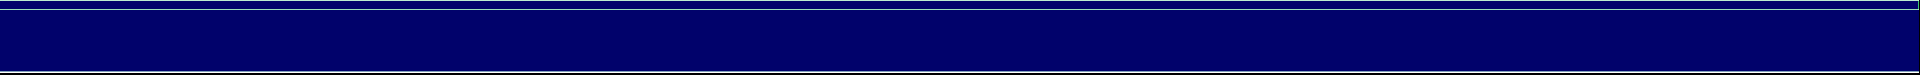
\includegraphics[height=0.9 true cm]{kekcsik.png}}

% ----------------------------------------------------------------------------------------------------------------------------------------

\begin{document}

\frame{\titlepage}

% ----------------------------------------------------------------------------------------------------------------------------------------

\begin{frame}[fragile,squeeze,allowframebreaks]
\frametitle{Introduction}
\begin{itemize}
\setlength{\parskip}{0pt}
\setlength{\itemsep}{0pt}
\item Dr. Gábor István FACSKÓ (\texttt{facsko.gabor@uni-obuda.hu}) – I answer e-mails.
\item MSc in Physics and Astronomy, BSc in Computer Science – Eötvös Loránd University (ELTE)
\item Assistant Professor, Óbuda University, Faculty of Electrical Engineering, Budapest
\item Senior Research Fellow, Wigner Research Centre for Physics, Department of Space Physics, Budapest, \url{http://wigner.hu/~facsko.gabor}
\item Research interests: Space Plasma Physics, Computational Magnetohydrodynamics (MHD), Spacecraft Data Analysis
\item Career:
\begin{itemize}
\item 2008: PhD in Physics, Eötvös Loránd University, Budapest – Data Analysis
\item 2008–2010: \textit{LPC2E/CNRS, Orléans, France} – Instrumentation
\item 2010–2013: \textit{Finnish Meteorological Institute, Helsinki, Finland} – MHD Simulations
\item 2014–2018: \textit{Institute of Earth Physics and Space Science, Sopron, Hungary} – MHD Simulations; teaching MSc students at ELTE (Budapest) and University of Sopron
\pagebreak
\item 2018–2020: \textit{European Space Agency (ESA), Darmstadt, Germany} – Management, ISSI International Team member
\item \textbf{2020–present: Wigner Research Centre for Physics, Department of Space Physics, Budapest} – Computational MHD, Data Analysis, teaching Space Plasma Physics for MSc students in Physics, Astronomy, and Geophysics
\item 2022–2024: \textit{Milton Friedman University, Budapest} – Teaching Linux/UNIX, C\#, Python, SQL, and \LaTeX\ for BSc IT students
\item 2024–2025: \textit{University of Pecs, Faculty of Sciences, Institute of Mathematics and Informatics, Pecs} – Teaching Linear Algebra and Python for BSc students in IT, Mathematics, Physics, and Chemistry; founder of Pannon SpaceLab
\item 2024–2025: \textit{NASA Goddard Space Flight Center, Greenbelt, MD, USA} – External Contractor (Visiting Scientist in 2016, 2017, 2023)
\item \textbf{2025–present: Obuda University, Faculty of Electrical Engineering, Budapest}~–~Teaching Physics for BSc Electrical Engineering students
\end{itemize}
\pagebreak
\item Supervision of 1 MSc in Physics, 1 BSc in Physics, 3 BSc IT, and 1 TDK student + \textbf{ 1 PhD student in Oulu}
\item Questions:
\begin{itemize}
\item You know what lecture, practice, signature, test, and exam mean, don’t you?
\item Do you know what a Scientific Students’ Conference (TDK) is?
\item Did you know that you can start a PhD after a BSc in the UK, USA, or Australia?
\end{itemize}
\item Special services:
 \begin{itemize}
\setlength{\parskip}{0pt}
\setlength{\itemsep}{0pt}
\item BSc and TDK thesis topics
\item Career advice (over 1400 contacts on Facebook and LinkedIn), \textbf{Master Plan}
\item Soft skills training (CVs, motivation letters, presentations, networking)
\end{itemize}
\item Lectures and practices recorded with OBS Studio and a mobile phone, uploaded to Moodle/Teams
\item All slides will be available on Moodle/Teams
\end{itemize}
\end{frame}



% ----------------------------------------------------------------------------------------------------------------------------------------

\begin{frame}[fragile,squeeze,allowframebreaks]
\frametitle{Course Objectives}
\small The physics curriculum is aligned with the university's traditions, requiring a high level of knowledge, building on previously acquired advanced mathematical skills, and aligning with the requirements of subsequent courses, which are based on physical concepts and ways of thinking. As a result, certain parts of the material are more detailed, while others are more comprehensive. The parts of the curriculum build on each other, both in terms of content and concepts, as well as in terms of thinking. The lectures present the theoretical material with a more detailed explanation of each important experiment, problem, or task. The calculation exercises deepen the most important areas related to the lecture material through the solution of specific tasks, based on the active participation of the students. The lecturer may deviate from the detailed syllabus by approximately 25\%. The aim of the course is to build and systematize the fundamentals of physics and fit them into a unified framework. With this knowledge, students will be able to understand the material of courses that teach modern technical knowledge. The course is intended for students in the following fields of study.
\pagebreak
\normalsize
\begin{itemize}
\setlength{\parskip}{0pt}
\setlength{\itemsep}{0pt}
\item \st{Motion of charged particles in electromagnetic fields.}
\item \textbf{Moving reference frames. Elements of special relativity.}
\item \textbf{Limits of the classical conceptual framework. Thermal radiation. Photoelectric effect. Compton effect. The dual nature of electromagnetic radiation. The dual nature of particles.}
\item \textbf{The classical theory of atomic structure (Rutherford, Franck-Hertz experiment, Bohr model, quantum numbers, Pauli exclusion principle).}
\item \textit{Elements of quantum mechanics. Heisenberg's uncertainty principle. The stationary Schrödinger equation and its applications.}
\item Physics of condensed matter. Metallic bonding. Electrical conduction in metals based on the free electron model and the wave model. Hall effect. Band theory of solids.
\pagebreak
\item Semiconductors. Elements of Fermi-Dirac statistics. Thermoelectric phenomena. Magnetic properties.  
\item Ferroelectricity. Piezoelectricity and electrostriction. Liquid crystals. Superconductivity.
\item Luminescence. Lasers. Basic knowledge of nuclear physics. Basic knowledge of particle physics.
\end{itemize}
\end{frame}

% ----------------------------------------------------------------------------------------------------------------------------------------

\begin{frame}[fragile,squeeze,allowframebreaks]
\frametitle{Requirements}
Students who fully comply with all of the points listed below during the semester may get a signature:
\begin{itemize}
\setlength{\parskip}{0pt}
\setlength{\itemsep}{0pt}
\item \st{The number of absences from lectures and exercises during the semester did not exceed the limit specified in the TVSZ (maximum 30\% of the total number of hours held).}
\item Correctly completed 3 of the 5 assigned homework assignments, submitted on time and in the required  format.
\item Achieved a score of at least 40\% on the midterm exam.
\item Extra credit: In addition to the homework assignments submitted during the semester, two more assignments can be submitted as extra credit. If the result of the assignment submitted in this way is correct, the student will receive +5 semester points per assignment. In this way, a maximum of +10 semester points can be earned with extra assignments, which will be included in the final semester score. The extra credit assignment can be submitted either during the two weeks of the given homework assignment or, at the latest, during the week designated for making up homework assignments (see below for make-up assignments in the 13th week of instruction).
 \pagebreak
\item Midterm exam: A poorly written or incorrect midterm exam with a score above 40\% cannot be corrected, i.e., it cannot be retaken for the purpose of correction. There is no retake exam. The score received for the extra credit assignment cannot be added to the score obtained on the midterm exam, i.e., the 40\% midterm exam score must be achieved solely from the midterm exam assignments.
\item Grades: Insufficient/Fail (1): 0-50\,\%, Sufficient/Pass (2): 51-60\,\%, Average (3): 61-75\,\%, Good (4): 76-90\,\%, Excellent (5): 91-\,\%.
\end{itemize}
\textbf{Recommended}\\
\textit{Richard~P.~Feyman, Robert~B.~Leighton, Matthew~Sands, The Feynman Lectures on Physics Vol 2-3, Addison-Wesley Publishin Company, 1977}
\end{frame}

% ----------------------------------------------------------------------------------------------------------------------------------------

\begin{frame}%[fragile,squeeze,allowframebreaks]
\frametitle{Thermal Radiations, Black Body}
\begin{itemize}
\setlength{\parskip}{0pt}
\item \underline{Definition (thermal radiation):} Radiation related to the temperature of bodies, covering the entire electromagnetic spectrum, is called \textit{thermal radiation}. (Cosmic Background Radiation, the Sun, stars)
\item \underline{Definition (spectral emissive power):} The spectral emissive power is measured by the magnitude of the portion of the intensity per unit solid angle corresponding to a unit wavelength interval. \ Symbol: E\ Unit: $W m^{-2}$\ Note: $E\left(\lambda, T\right)$, where $\lambda$ is the wavelength [m] $T$ is the temperature [K]. 
\item \underline{Definition (black body):} A body that absorbs all incident radiation (perfect absorber) and emits all electromagnetic radiation to the maximum possible extent (perfect emitter) is called a \textit{black body}.
\item Consequence: It serves as a useful model for formulating the laws of radiation.
\item Here, we deal with the description of thermal radiations of a black body.
\end{itemize}
\end{frame}

% ----------------------------------------------------------------------------------------------------------------------------------------

\begin{frame}%[fragile,squeeze,allowframebreaks]
\frametitle{The Stefan-Boltzmann Radiation Law}
\begin{itemize}
\setlength{\parskip}{0pt}
\item The radiation of the absolut black body
\item Here, P [W] is the heat power, A [$m^{2}$] is the surface, T [K] is the absolute temperature.
\item Therefore: $P\sim T^{4}$
\item Or: $P\sim A T^{4}$
\item Adding the Stefan-Boltzmann coefficient:  $P\sim \sigma A T^{4}$ where $\sigma=5.67\cdot 10^{-8}Wm^{-2}K^{4}$.
\item \underline{Stefan–Boltzmann Radiation Law:} A black body with surface area ``A'' emits, per unit time, a thermal power proportional to the fourth power of its absolute temperature.
\end{itemize}
\end{frame}

% ----------------------------------------------------------------------------------------------------------------------------------------

\begin{frame}[fragile,squeeze,allowframebreaks]
\frametitle{Wien's Displacement Law}
\includegraphics[width=0.55\textwidth]{images-20251006/Wiens_law.svg.png}
\pagebreak
\begin{itemize}
\setlength{\parskip}{0pt}
\item \underline{Wien's displacement law:} The law describes the relationship between the wavelength $\lambda_{max}$ corresponding to the maximum of the black body’s spectral emissive power and its absolute temperature. The wavelength $\lambda_{max}$ corresponding to the maximum of the spectral emissive power and the absolute temperature $T$ are inversely proportional quantities.
$$\lambda_{max}\cdot T = const,$$
where $const = 2.88 \cdot 10^{-3} m K$.
\item It gives a curve consistent with experimental results only for short wavelengths and low temperatures.
\end{itemize}
\end{frame}

% ----------------------------------------------------------------------------------------------------------------------------------------

\begin{frame}[fragile,squeeze,allowframebreaks]
\frametitle{The Rayleigh–Jeans Formula}
\begin{itemize}
\setlength{\parskip}{0pt}
\item Applying the classical physics principle of equal energy distribution, Rayleigh and Jeans attempted to determine the specific form of the spectral energy density of the radiation field, $E\left(f, T\right)$ or $E\left(\lambda, T\right)$.
\item Rayleigh–Jeans formula:
$$E\left(f,T\right)=\frac{8\pi}{c^{3}}f^{2}kT,$$
where $T$ is the temperature, $f$ is the frequency, $c$ is the speed of light, and $k = 1.38 \cdot 10^{-23} , m^{2} kg , s^{-2} K^{-1}$ is the Boltzmann constant.
\item After transforming $f \rightarrow \lambda$, we obtain the Rayleigh–Jeans law:
$$E\left(\lambda,T\right)=\frac{8\pi k}{\lambda^{5}}\lambda T,$$
where $\lambda$ is the wavelength.
\pagebreak
\item This law gave results consistent with experimental data only in the longer-wavelength region of the spectrum. In the shorter-wavelength region, it showed large deviations from experimental results.
\item For very short wavelengths, the Rayleigh–Jeans law predicts unrealistically large spectral energy densities. In other words:
$$\lim_{\lambda\rightarrow 0}\left(\frac{8\pi k}{\lambda^{5}}\lambda T\right)=\infty.$$
\item This phenomenon is known as the \textit{ultraviolet catastrophe}.
\pagebreak
\item Summary
\begin{center}
  \includegraphics[width=0.6\textwidth]{images-20251006/wien_planckt.png}
\end{center}
\end{itemize}
\end{frame}

% ----------------------------------------------------------------------------------------------------------------------------------------

\begin{frame}[fragile,squeeze,allowframebreaks]
\frametitle{The Planck Radiation Law}
\begin{itemize}
\setlength{\parskip}{0pt}
\item After the discovery of the “partial laws” of Wien and Rayleigh–Jeans, identifying the fundamental law that perfectly matched the experimental results — that is, determining the analytical form and theoretical interpretation of the function $E\left(\lambda,T\right)$ — remained unsuccessful for quite some time, despite the efforts of many prominent physicists.
\item Max Planck, through trial and error, succeeded in combining the two formulas in such a way that both the Wien and the Rayleigh–Jeans laws emerged as limiting cases.
\item His relation correctly describes the intensity of radiation across the entire spectral range.
\item Subsequently, Planck developed a derivation based on purely theoretical reasoning, which also produced the correct formula. However, this derivation required a revolutionary new assumption that broke away from classical physics.
\item \underline{Planck’s Hypothesis 1:} Thermal radiation (electromagnetic waves) is produced by small vibrating oscillators. The possible energy states of such an oscillator cannot take arbitrary or continuously varying values but only the following discrete ones:
$$\epsilon, 2\epsilon, 3\epsilon, 4\epsilon, \dots$$
\item Thus, in the $n$th state of an oscillator, the energy can be expressed as:
$$\epsilon_{n}=n\epsilon,$$
where $n\in\mathbb{N}^{+}$.
\item \underline{Planck’s Hypothesis 2:} Oscillators transition abruptly between possible states (‘‘jumping over’’ intermediate ones), while emitting or absorbing the corresponding energy difference. The emission or absorption of radiant energy therefore occurs in discrete packets, or \textit{quanta} of energy. According to Planck, the energy quantum is proportional to the frequency of the emitted or absorbed vibration, that is:
$$\epsilon\sim f,$$
or
$$\epsilon=h\cdot f,$$
where $f$ is the frequency and $h = 6.626176\cdot 10^{-34} J s$ is the \textbf{Planck constant}.
\item The constant $h$ is a proportionality factor — a universal constant named the Planck constant in honor of Max Planck.
\pagebreak
\item Planck himself called this constant the \textit{quantum of action}.
\item The \underline{Planck Radiation Law} can be expressed mathematically as follows:
$$E\left(f,T\right)=\frac{8\pi h f^{3}}{c^{3}}\frac{1}{e^{\frac{h f}{k T}}-1},$$
and
$$E\left(\lambda,T\right)=\frac{8\pi c h}{\lambda^{5}}\frac{1}{e^{\frac{h c}{\lambda k T}}-1},$$
where $c$ [m/s] is the speed of light in vacuum, $f$ [1/s] is the frequency of the radiation, $\lambda$ [m] is the wavelength, $k$ is the Boltzmann constant, $T$ [K] is the absolute temperature, and $h$ is the Planck constant.
\end{itemize}
\pagebreak
\begin{center}
  \includegraphics[width=0.62\textwidth]{images-20251006/planck.png}
\end{center}
\end{frame}

% ----------------------------------------------------------------------------------------------------------------------------------------

\begin{frame}[fragile,squeeze,allowframebreaks]
\frametitle{The Photoelectric Effect – Preliminary Experimental Results}
\begin{itemize}
\setlength{\parskip}{0pt}
\item \underline{Hertz’s observation:} In 1887, Hertz discovered that ultraviolet light facilitates spark discharge between metal electrodes.
\item \underline{The Hallwachs–Stoletov effect:}
\begin{center}
\includegraphics[width=0.4\textwidth]{images-20251006/hallwachs.png}
\end{center}
In 1888, Hallwachs and Stoletov found that ultraviolet radiation releases negative charges from a negatively charged metal plate.
\pagebreak
\item \underline{Observations by P. Lenard and J.J. Thomson – the external photoelectric effect:} In 1898, P. Lenard and J.J. Thomson, through vacuum experiments, measured the specific charge of the particles emitted from metals under the influence of light and determined that these emitted particles are electrons.
\end{itemize}
\end{frame}

% ----------------------------------------------------------------------------------------------------------------------------------------

\begin{frame}%[fragile,squeeze,allowframebreaks]
  \frametitle{The Photoelectric Effect - Nobel Prize, Albert EINSTEIN, 1905}
\begin{center}
  \includegraphics[width=0.65\textwidth]{images-20251006/photo.png}
\end{center}
\end{frame}

% ----------------------------------------------------------------------------------------------------------------------------------------

\begin{frame}[fragile,squeeze,allowframebreaks]
\frametitle{Basic Experiments and results of the Photoelectric Effect}
\begin{center}
\includegraphics[width=0.52\textwidth]{images-20251006/photo_exp.png}
\end{center}
\pagebreak
\begin{itemize}
\setlength{\parskip}{0pt}
\item The maximum velocity $v_{max}$ of the photoelectrons, or the corresponding value of $V_{r}$, is independent of the light intensity and depends only on the frequency $f$ (or the wavelength $\lambda$) of the incident light.
\item When a given photocathode is illuminated with light of different frequencies $f$, the photoelectric current $I_{f}$ appears only above a certain threshold frequency $\mu_{h}$ (characteristic of the photocathode), or equivalently, when the wavelength of the incident light is shorter than the threshold wavelength $\lambda_{h}$.
\item The number of emitted electrons is proportional to the intensity of the incident light.
\item The photoelectric effect is an “inertia-free” phenomenon — that is, the electrons are emitted simultaneously with the incidence of the radiation (within $10^{-8}$ s).
\end{itemize}
\vskip -20 pt
\begin{center}
\includegraphics[width=0.20\textwidth]{images-20251006/photo_exp2.png}
\end{center}
\end{frame}

% ----------------------------------------------------------------------------------------------------------------------------------------

\begin{frame}%[fragile,squeeze,allowframebreaks]
  \frametitle{Creation of X-rays}
\begin{center}
  \includegraphics[width=0.45\textwidth]{images-20251006/xray.png}
\end{center}
\end{frame}

% ----------------------------------------------------------------------------------------------------------------------------------------

\begin{frame}[fragile,squeeze,allowframebreaks]
  \frametitle{Compton Scattering}
\begin{center}
  \includegraphics[width=0.6\textwidth]{images-20251006/compton.png}
\end{center}
\pagebreak
\begin{itemize}
\setlength{\parskip}{0pt}
\item Derivation of the Compton formula: \begin{center}
\includegraphics[width=0.3\textwidth]{images-20251006/compton2.png}
\end{center}
\item Writing down the law of momentum conservation: $$p_{e}^{2}=p^{2}+p_{0}^{2}-2p_{0}p\cos\alpha$$ (law of cosines)
\pagebreak
\item Writing down the law of energy conservation: $$ h  f_{0} + m_{0} c^{2} = h f + W_{e},$$ where $f_{0}$ is the original frequency, $f$ is the frequency of the scattered radiation, $m_{0}c^{2}$ is the rest energy of the electron, and $W_{e}$ is the energy of the electron after the collision. 
\end{itemize}
\end{frame}

% ----------------------------------------------------------------------------------------------------------------------------------------

\begin{frame}%[fragile,squeeze,allowframebreaks]
\frametitle{The Dual Nature of Electromagnetic Radiation}
\begin{itemize}
\setlength{\parskip}{0pt}
\item Particle nature
\begin{itemize}
\item Thermal radiation
\item Photoelectric effect
\item Compton effect
\end{itemize}
\item Wave nature
\begin{itemize}
\item Interference
\item Diffraction, refraction, reflection
\end{itemize}
\item Model: Wave model and particle model
\item Electromagnetic radiation exhibits a dual nature.
\end{itemize}
\end{frame}

% ----------------------------------------------------------------------------------------------------------------------------------------

\begin{frame}
%\frametitle{Minden jó, ha a vége jó}

\vfill
\begin{center}
\textbf{\huge The End}

\bigskip
Thank you for your attention!
\end{center}
\vfill
\end{frame}

\end{document}
